\documentclass{sig-alternate}

\usepackage{url}
\usepackage{amsmath}
\usepackage{graphicx}
\usepackage{subfigure}
\usepackage{threeparttable}
\usepackage{pdflscape}
\usepackage{array}
\usepackage{color}

\begin{document}

\title{The Bug Catalog of the Maven Ecosystem}

\numberofauthors{1}

%\author{
%% 1st. author
%\alignauthor
%Dimitris Mitropoulos\\
%       \affaddr{Athens University of Economics and Business}\\
%       \affaddr{Department of Management Science and Technology}\\
%       \email{dimitro@aueb.gr}
%% 2nd. author
%\alignauthor Vassilios Karakoidas\\
%       \affaddr{Athens University of Economics and Business}\\
%       \affaddr{Department of Management Science and Technology}\\
%       \email{bkarak@aueb.gr}
%% 3rd. author
%\alignauthor Panos Louridas\\
%       \affaddr{Athens University of Economics and Business}\\
%       \affaddr{Department of Management Science and Technology}\\
%       \email{louridas@aueb.gr}
%\and  % use '\and' if you need 'another row' of author names
%% 4th. author
%\alignauthor Georgios Gousios\\
%       \affaddr{Delft University of Technology}\\
%       \affaddr{Software Engineering Research Group}\\
%       \email{G.Gousios@tudelft.nl}
%% 5th. author
%\alignauthor Diomidis Spinellis\\
%       \affaddr{Athens University of Economics and Business}\\
%       \affaddr{Department of Management Science and Technology}\\
%       \email{dds@aueb.gr}
%}

\def\aueb{\textsuperscript{*}}
\def\tud{\textsuperscript{\dag}}

\author{
  Dimitris Mitropoulos\aueb \and Vassilios Karakoidas\aueb \and Panos Louridas\aueb \and Georgios Gousios\tud \and Diomidis Spinellis\aueb \\
  \begin{tabular}{ccc}
  \affaddr{\aueb Department of Management Science and Technology} & & \affaddr{\tud Software Engineering Research Group}\\
    \affaddr{\aueb Athens University of Economics and Business} & & \affaddr{\tud Delft University of Technology}\\
   \affaddr{Athens, Greece} & & \affaddr{Delft, the Netherlands}\\
   \email{\{dimitro,bkarak,louridas,dds\}@aueb.gr}& & \email{g.gousios@tudelft.nl} \\
  \end{tabular}
}

\maketitle
\begin{abstract}
Examining software ecosystems can provide the research community
with useful information. To examine the ecosystem of
the Maven Central Repository (approximately 265{\sc gb} of data),
we performed an experiment where we statically analyzed the
repository to detect its software bugs. For our analysis we
used FindBugs, a tool that examines Java bytecode to detect
numerous types of bugs. In this paper we present our data collection
experiment and show our findings regarding software evolution.
\end{abstract}

\category{D.2.4}{Software Engineering}{Software/Program Verification}[Statistical methods]
\category{D.2.5}{Software Engineering}{Testing and Debugging}[Code inspections and walk-throughs]
\category{D.2.7}{Software Engineering}{Distribution, Maintenance, and Enhancement}[Version control]

\terms{Static Analysis, Software Ecosystems}

\keywords{Maven Repository, FindBugs, Software Bugs}

\section{Introduction}
\label{sec:intro}

A software ecosystem can be seen as a collection of software projects,
which are developed and co-evolve in the same environment~\cite{LL10}.
Components can be interdependent and have multiple versions.
Examples of such ecosystems include Python's
{\sc p}y{\sc py}\footnote{\url{http://pypy.org/}}
(Python Package Index), Perl's
{\sc cpan}\footnote{\url{http://www.cpan.org/}}
(Comprehensive Perl Archive Network), Ruby's
RubyGems\footnote{\url{http://rubygems.org/}}
and the Maven Central Repository.\footnote{\url{http://mvnrepository.com/}}

Maven is a build automation tool used primarily for Java projects and it is
hosted by the Apache Software Foundation.\footnote{\url{http://maven.apache.org/}}
It uses {\sc xml} to describe the software project being built, its dependencies
on other external modules, the build order, and required plug-ins.
To build a software component, it dynamically downloads Java libraries
and Maven plug-ins from the Maven central repository,
and stores them in a local cache. The repository can be updated with
new projects and also with new versions of existing projects
that can depend on other versions.

To statically analyze the Maven repository
we used {\it FindBugs},\footnote{\url{http://findbugs.sourceforge.net/}}
a static analysis tool that examines bytecode to detect software bugs
and has already been used in research~\cite{AP10,SHP06}.
Specifically, we ran FindBugs on all the project versions of all
the projects that exist in the repository
to identify all bugs contained in it.

In this paper we present: a) the experiment performed to obtain the
collection of the metric results that the FindBugs tool produces 
for every project version of the repository (115,214 {\sc jar}s)
and b) how researchers can use the dataset and include it in their research.

\begin{table}
\centering
\begin{tabular}{l r}
\hline
Measurement & Value\\
 \hline
Projects & 17,505\\
Versions (total) & 115,214\\
Min (versions per project) & 1\\
Max (versions per project) & 338\\
Mean (versions per project) & 6.58\\
Median (versions per project) & 3\\
Range (over versions) & 337\\
1$^{st}$ Quartile (over versions) & 1\\
3$^{rd}$ Quartile (over versions) & 8\\
\hline
\end{tabular}
\caption{Descriptive statistic measurements for the Maven repository.}
\label{tbl:repository}
\end{table}

\section{Data Collection Experiment}
\label{sec:exp}

First, we scanned the Maven repository only
for appropriate {\sc jar}s and created a list that included them.
This is because FindBugs analyzes applications written in Java,
and the Maven repository hosts projects from
languages other than Java such as Scala, Groovy,
Clojure, etc. Thus we filtered out such projects.
In particular, we obtained a snapshot (January 2012) of
the repository and handled it locally to retrieve a list of all
the names of the project versions that existed in it.
The statistic measurements concerning the repository can be seen in 
Table~\ref{tbl:repository}.

With the {\sc jar} list at hand, we created a series of processing tasks
and added them to a task queue mechanism (a Rabbit{\sc mq} message
broker). Then we executed twenty five workers (custom Python scripts)
that checked out tasks from the queue, processed each project version
and stored the results to the data
repository (a Mongo{\sc db} database system).

A typical processing cycle of a worker included the following steps: after
the worker spawned, it requested a task from the queue. This task contained
the {\sc jar} name, which was typically a project version that was downloaded locally.
First, specific {\sc jar} metadata were calculated and stored. Such metadata included
its size, its dependencies, and a number that represented the chronological order of the
release. This order was derived from an {\sc xml} file that
accompanies every project in the Maven repository called {\it
maven-metadata.xml}. Then, FindBugs was invoked by the worker and its results were
also stored in the data repository. 
FindBugs separates software bugs into nine
categories\footnote{\url{http://findbugs.sourceforge.net/bugDescriptions.html}}
(including Bad Practice, Security, Performance and others)
and reports bug collections that include all the bugs discovered in a
{\sc jar} file. For every registered bug, there are numerous accompanying features
like the class, the method and the line that the bug was found.
When the task was completed the queue
was notified and the next task was requested. A schematic representation of
the data processing architecture can be seen in Figure~\ref{fig:arch}.

\begin{figure} [h]
  \begin{center}
    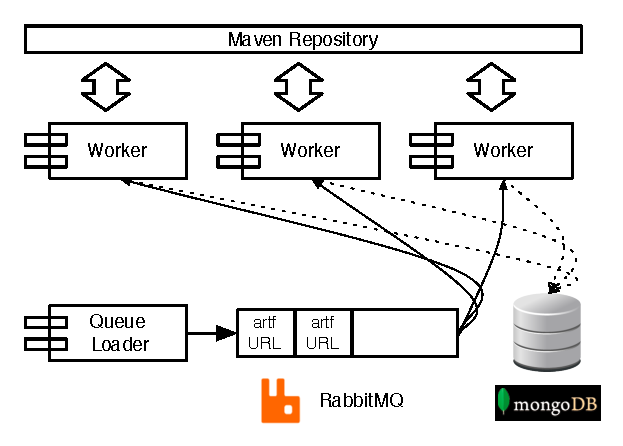
\includegraphics[scale=0.73]{figures/arch.pdf}
  \end{center}
  \caption{The data processing architecture.}
  \label{fig:arch}
\end{figure}

\section{Data and Findings}
\label{sec:find}

As we mentioned earlier our data was stored in a
Mongo{\sc db} database, thus all the data were 
converted to the {\sc json} format. FindBugs output data is in {\sc xml} format. The conversion was a straight forward mapping
of the {\sc xml} elements to {\sc json} objects. In addition, to the FindBugs data, we added a metadata section, which contained
several additional information regarding the jar file that has been processed (Table~\ref{tbl:metadata-description}). The following listing contains an excerpt:

\begin{verbatim}
{"JarMetadata": {"jar_filename": "",
                 "jar_size": "",
                 "version": "",
                 "version_list": "",
                 "artifact_id": "",
                 "group_id": "",
                 "dependencies": ""}, 
 "BugCollection": { /* FindBugs data */ }}
\end{verbatim}

Since Mongo{\sc db} provides a rich query interface, it was easy to either create
queries to find out basic information like:
``how many bad practice bugs exist in the repository", or
create scripts that can help us capture correlations
that could provide valuable findings. Figure~\ref{fig:bug-per} shows how software 
bugs are distributed among the repository.

\begin{table}
\centering
\caption{Jar metadata description}
\label{tbl:metadata-description}
\begin{tabular}{l p{5.0cm}}
 \hline
\verb|jar_filename| & JAR's filename\\
\verb|jar_size| & The size of the JAR file\\
\verb|version| & The version of the project in Maven repository\\
\verb|version_list| & A list of project's version numbers\\
\verb|artifact_id| & The artifact id of the project in Maven repository\\
\verb|group_id| & The group id of the project in Maven repository\\
\verb|dependencies| & List of all dependencies for the project\\
 \hline
 \end{tabular}
\end{table}

\begin{figure}[t]
	\centering
	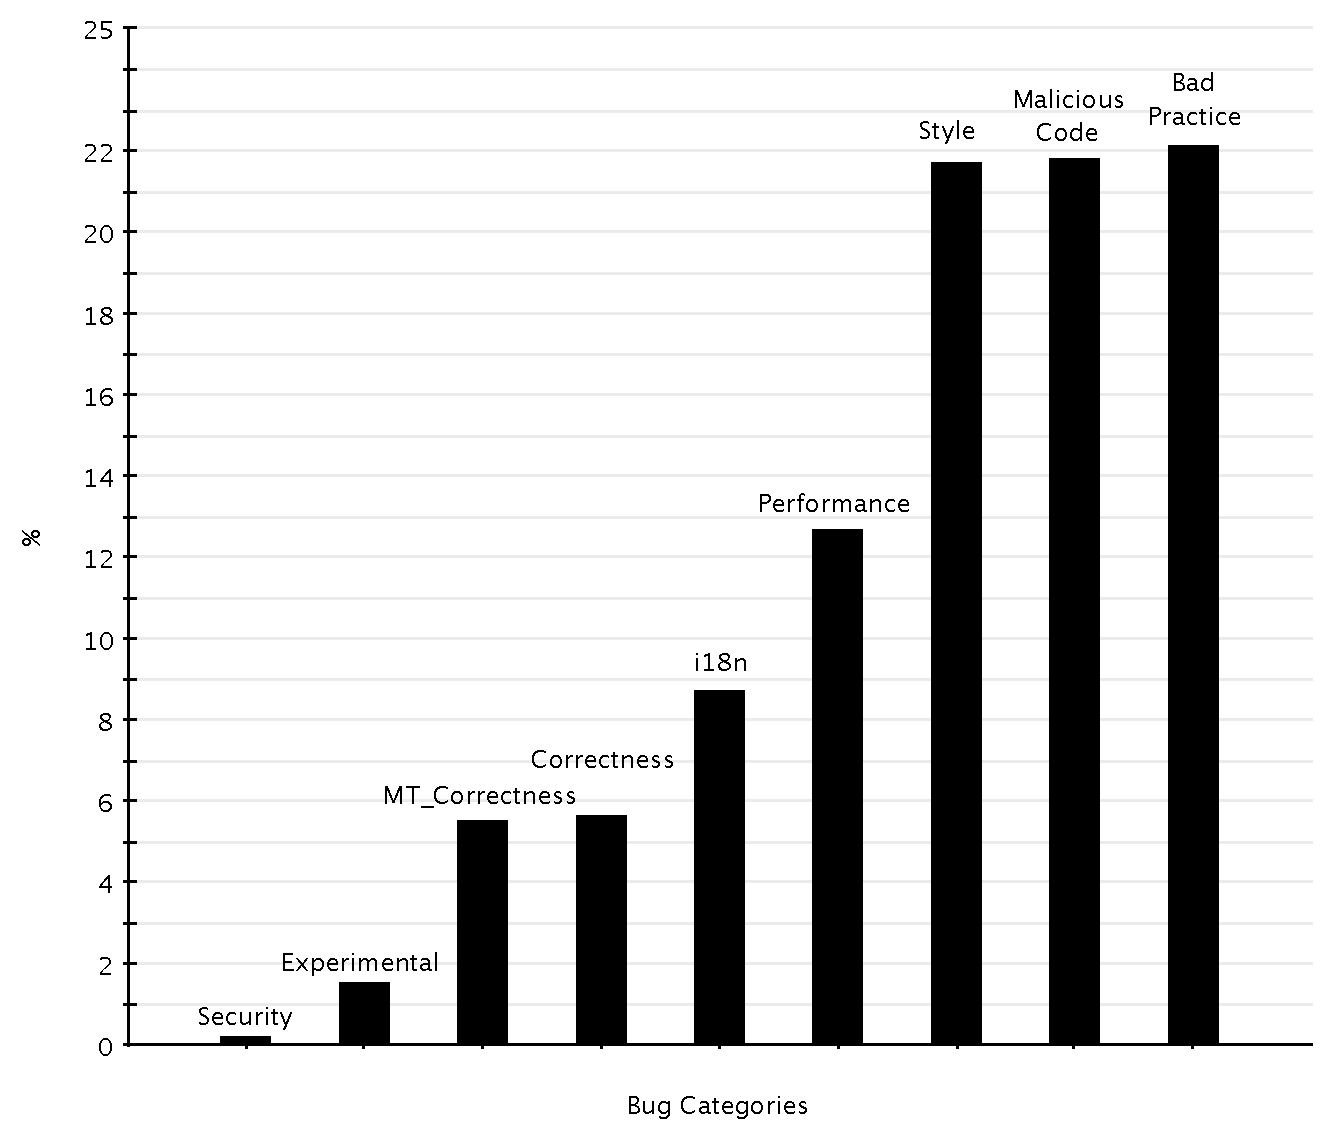
\includegraphics[scale=0.38]{figures/bug_percent}
	\caption{Bug percentage in Maven repository.}
	\label{fig:bug-per} 
\end{figure}

\begin{figure}
  \centering
  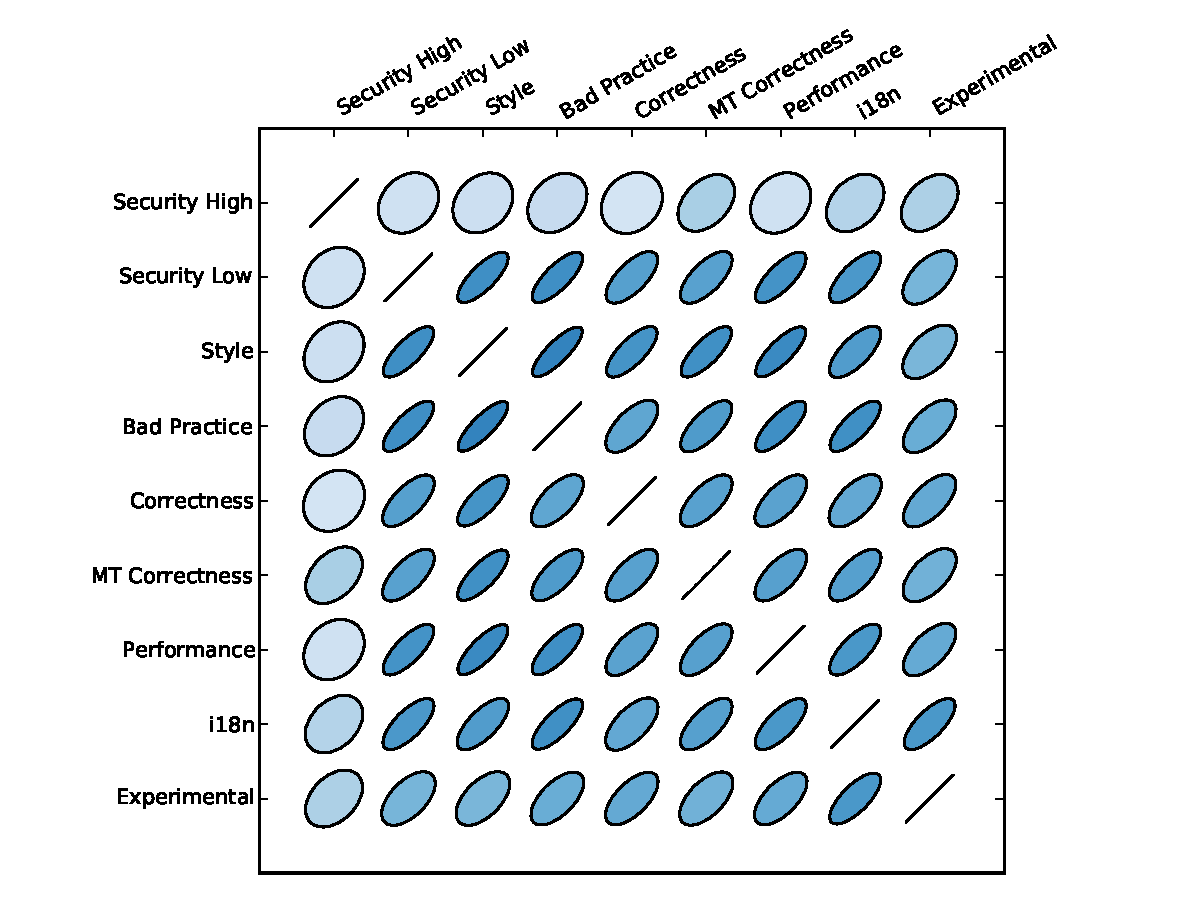
\includegraphics[scale=0.43]{corrplot.pdf}
  \caption{Correlation matrix plot for bug categories.}
  \label{fig:corrplot}
\end{figure}

\section{Related Work}
\label{sec:rel}

The Maven ecosystem has been previously analyzed by
Raemaekers et al.~\cite{RDV13}
to produce the {\it Maven dependency dataset}.
Apart from basic information like individual methods, classes,
packages and lines of code for every {\sc jar}, this dataset
also includes a database with all the
connections between the aforementioned elements.

\section{Conclusions}
\label{sec:conc}

\bibliographystyle{abbrv}
\bibliography{msr}  
\end{document}
